\documentclass[11pt]{article}
\usepackage[margin=1in]{geometry}
\usepackage{amsmath,amssymb,amsthm,mathtools}
\usepackage{booktabs,tabularx,array}
\usepackage{microtype}
\usepackage{xcolor}
\usepackage{tikz}
\usepackage[hidelinks]{hyperref}
\allowdisplaybreaks[2]

\newtheorem{theorem}{Theorem}
\newtheorem{proposition}[theorem]{Proposition}
\newtheorem{lemma}[theorem]{Lemma}
\newtheorem{corollary}[theorem]{Corollary}
\theoremstyle{definition}
\newtheorem{definition}[theorem]{Definition}
\theoremstyle{remark}
\newtheorem{remark}[theorem]{Remark}

\newcommand{\Bd}{\mathrm{Bd}}
\newcommand{\dB}{\mathrm{dB}}
\newcommand{\Rsim}{R_{\mathrm{sim}}}
\newcommand{\Rhyb}{R_{\mathrm{hyb}}}
\newcommand{\eps}{\varepsilon}
\newcommand{\Prob}{\mathbb P}

\title{Simultaneous amplification beyond fitness three halves}
\author{Alec Kriebel\\Independent Researcher}
\date{August 8, 2026}

\begin{document}
\maketitle

\begin{abstract}
We study fixation from a uniformly random single mutant on finite connected
loopless undirected weighted graphs under both Birth--death (Bd) and
death--Birth (dB) Moran updating.  Let $\Rhyb$ be the unique root in
$(3/2,151/100)$ of
\[
 R^6-8R^5+22R^4-30R^3+21R^2-6R+1.
\]
We construct one fitness-independent graph family which, for every fixed
$1<r<\Rhyb$, strictly amplifies fixation under both rules for all
sufficiently large populations.  Numerically,
$\Rhyb=1.5028569127905696\ldots$, and hence
$\Rsim\geq\Rhyb>3/2$.

The graph combines a large clique, a dilute collection of hub pendants, and
a dilute collection of internally heavy two-vertex satellites coupled to
the clique through positive weak edges.  We first derive the exact finite
weak-cut trace.  We then control establishment and the entire path to
fixation, obtaining the normalized corrections
\[
 B(r)=\frac{2(\sigma-1)}{1+\sigma(r^2-1)}
       +\frac{\lambda}{r-1},\qquad
 D(r)=\frac{2\{r(2-r)-\sigma\}}{\sigma+2r(r-1)}-\lambda.
\]
Optimizing the interval on which both are positive gives the displayed
sextic.  Independent labelled-event and symbolic verifiers audit the
lumping, trace coefficients, root isolation, and tangency.

This disproves the proposed exact threshold $3/2$.  We also exactly refute
every graph-independent convex affine endpoint separator.  The unrestricted
exact value of $\Rsim$ remains open.
\end{abstract}

\begin{center}
\fbox{\parbox{0.91\textwidth}{\centering
\textbf{Scope.}  This paper proves the lower bound
$\Rsim\geq\Rhyb=1.5028569127905696\ldots>3/2$ and the exact threshold of
the displayed two-mechanism dilute hybrid.  It does \emph{not} prove a
universal upper bound or determine the exact unrestricted value of
$\Rsim$.}}
\end{center}

\section*{Author summary}

The two standard update orders in evolutionary graph theory often reward
opposite structural features.  We combine two small effects at a vanishing
population proportion.  Internally heavy pairs improve death--Birth
fixation but slightly reduce Birth--death fixation.  Hub pendants have the
opposite effect.  Their proportions can be balanced so that both net
effects are positive, even at fitness $3/2$ and on a short interval above
it.  Exact optimization produces an algebraic endpoint near $1.5028569$.
The weak links are chosen uniformly over a growing fitness interval, so the
graph sequence is fixed before fitness is quantified.

\section{Introduction}

A population structure is a simultaneous amplifier at fitness $r$ when it
raises uniformly initialized fixation probability, relative to the complete
graph of the same order, under both Bd and dB updating.  The asymptotic
question has the quantifier order
\[
 \exists\{G_t\}\ \forall r\in(1,R)\ \exists t_0(r)\
 \forall t\geq t_0(r).
\]
The graphs and weights may depend on $t$, but not on $r$.

Svoboda, Joshi, Tkadlec, and Chatterjee constructed simultaneous amplifiers
on the interval $1<r<1.2$ \cite{Svoboda2024}.  A separate center--triangle
construction subsequently established $\Rsim\geq3/2$, while that particular
family suppresses at the endpoint.  The latter fact suggested, but did not
prove, that $3/2$ might be the universal phase boundary.

The present construction crosses that boundary.  The mechanism is a
dilute linear combination of two rigorously traced modules.  Its exact
optimization also identifies the best threshold within this two-mechanism
leading regime.  Two endpoint proof programs are thereby closed: universal
impossibility at $3/2$ is false, and an exact order-$22$ graph rules out
every fixed convex affine separator of the two normalized endpoint
probabilities.

\section{Model, baselines, and threshold}

Let $G=(V,w)$ be finite, connected, loopless, undirected, and weighted:
\[
 w_{uv}=w_{vu}\geq0,\qquad w_{uu}=0,\qquad
 d_u:=\sum_vw_{uv}>0.
\]
A state is a mutant set $S\subseteq V$.  Mutants have fitness $r>1$ and
residents fitness one.  Under Bd, a parent is selected proportional to
fitness and then a replacement target proportional to edge weight.  Under
dB, a uniformly chosen target dies and then a parent is selected
proportional to fitness times edge weight.  Thus, with
$F(S)=|V|+(r-1)|S|$,
\begin{align}
 P_{\Bd}(S,S\cup\{v\})
 &=\frac r{F(S)}\sum_{u\in S}\frac{w_{uv}}{d_u},
 &&v\notin S,\\
 P_{\Bd}(S,S\setminus\{v\})
 &=\frac1{F(S)}\sum_{u\notin S}\frac{w_{uv}}{d_u},
 &&v\in S,\\
 P_{\dB}(S,S\cup\{v\})
 &=\frac1{|V|}
 \frac{r\sum_{u\in S}w_{uv}}
 {r\sum_{u\in S}w_{uv}+\sum_{u\notin S}w_{uv}},
 &&v\notin S,\\
 P_{\dB}(S,S\setminus\{v\})
 &=\frac1{|V|}
 \frac{\sum_{u\notin S}w_{uv}}
 {r\sum_{u\in S}w_{uv}+\sum_{u\notin S}w_{uv}},
 &&v\in S.
\end{align}
The fixation function $h_U$ is the unique harmonic solution with boundary
values zero at $\varnothing$ and one at $V$.  We use
\[
 \rho_U(G,r)=\frac1{|V|}\sum_{v\in V}h_U(\{v\}),
 \qquad U\in\{\Bd,\dB\}.
\]

Direct solution of the one-dimensional complete-graph count chains gives
\begin{align}
 \rho_{\Bd}(K_n,r)
 &=\frac{1-r^{-1}}{1-r^{-n}},\\
 \rho_{\dB}(K_n,r)
 &=\frac{n-1}{n}\frac{1-r^{-1}}{1-r^{-(n-1)}}.
\end{align}
Both converge, for fixed $r>1$, to
\[
 p(r):=1-\frac1r.
\]

\begin{definition}
$\Rsim$ is the supremum of all $R>1$ for which one
fitness-independent family $\{G_t\}$, with $|V(G_t)|\to\infty$, satisfies
\[
 \rho_{\Bd}(G_t,r)>\rho_{\Bd}(K_{|V(G_t)|},r),\qquad
 \rho_{\dB}(G_t,r)>\rho_{\dB}(K_{|V(G_t)|},r)
\]
for every fixed $r\in(1,R)$ and every sufficiently large $t$.
\end{definition}

\section{The dilute pair--pendant hybrid}

Let
\[
 P(R)=R^6-8R^5+22R^4-30R^3+21R^2-6R+1
\]
and let $\Rhyb$ be its unique root in $(3/2,151/100)$.  Define
\begin{align}
 \sigma_*&=
 \frac{-\Rhyb^3+4\Rhyb^2-3\Rhyb-1}{2(\Rhyb-1)},\\
 \lambda_*&=
 \frac{2(\Rhyb-1)(1-\sigma_*)}
 {1+\sigma_*(\Rhyb^2-1)}.
\end{align}
Exact root isolation gives
\[
 \Rhyb=1.5028569127905696\ldots,\quad
 \sigma_*=0.1306772822870484\ldots,\quad
 \lambda_*=0.7508064830318805\ldots .
\]

For $t\geq2$, put
\[
 q_t=t,\qquad m_t=\lfloor\lambda_*t\rfloor,\qquad C_t=t^4,
\qquad n_t=C_t+m_t+2q_t.
\]
The graph contains:
\begin{enumerate}
\item a unit-weight clique on $C_t$ vertices, one designated as the hub;
\item $m_t$ unit-weight leaves adjacent only to the hub;
\item $q_t$ disjoint two-vertex satellites, each with internal edge weight
      $W_t=C_t/\sigma_*$;
\item an edge of common weight $\eps_t>0$ from every satellite vertex to
      every clique vertex.
\end{enumerate}
There are no other edges.  In particular, there are no satellite--satellite
edges.

\begin{figure}[ht]
\centering
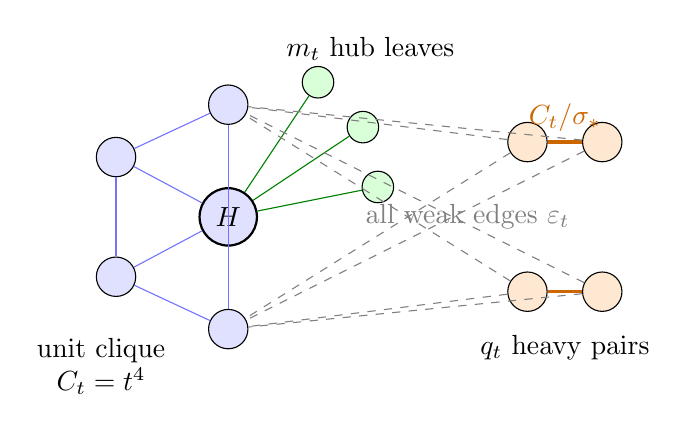
\begin{tikzpicture}[scale=0.95,
 core/.style={circle,draw,fill=blue!12,minimum size=5mm},
 pair/.style={circle,draw,fill=orange!18,minimum size=5mm},
 leaf/.style={circle,draw,fill=green!15,minimum size=4mm}]
\node[core,thick] (h) at (0,0) {$H$};
\node[core] (c1) at (-1.5,0.8) {};
\node[core] (c2) at (-1.5,-0.8) {};
\node[core] (c3) at (0,1.5) {};
\node[core] (c4) at (0,-1.5) {};
\foreach \x/\y in {h/c1,h/c2,h/c3,h/c4,c1/c2,c1/c3,c2/c4,c3/c4}
 \draw[blue!55] (\x)--(\y);
\node[leaf] (l1) at (1.2,1.8) {};
\node[leaf] (l2) at (1.8,1.2) {};
\node[leaf] (l3) at (2.0,0.4) {};
\foreach \x in {l1,l2,l3}\draw[green!50!black] (h)--(\x);
\node[pair] (a1) at (4.0,1.0) {};
\node[pair] (a2) at (5.0,1.0) {};
\node[pair] (b1) at (4.0,-1.0) {};
\node[pair] (b2) at (5.0,-1.0) {};
\draw[orange!80!black,very thick] (a1)--node[above] {$C_t/\sigma_*$}(a2);
\draw[orange!80!black,very thick] (b1)--(b2);
\foreach \x in {a1,a2,b1,b2}{
 \draw[gray,dashed] (\x)--(c3);
 \draw[gray,dashed] (\x)--(c4);
}
\node[align=center] at (-1.7,-2.0) {unit clique\\$C_t=t^4$};
\node[align=center] at (1.9,2.25) {$m_t$ hub leaves};
\node[align=center] at (4.5,-1.75) {$q_t$ heavy pairs};
\node[gray] at (3.2,0) {all weak edges $\eps_t$};
\end{tikzpicture}
\caption{Schematic of the dilute hybrid.  Dashed lines represent all
satellite--clique edges, not only those drawn.}
\label{fig:hybrid}
\end{figure}

To define the positive coupling without reference to a subsequently chosen
fitness, let
\[
 I_t=[1+1/t,\Rhyb-1/t]
\]
when this interval is nonempty.  Let $\rho^0_{U,t}$ denote the finite
separated trace defined in Section~\ref{sec:trace}.  Choose $e_t$ to be the
least positive integer such that, for $\eps_t=2^{-e_t}$,
\[
 \sup_{r\in I_t}\frac{n_t}{q_t}
 \left|
 \frac{\rho_U(G_t(\eps_t),r)}{\rho_U(K_{n_t},r)}
 -\frac{\rho^0_{U,t}(r)}{\rho_U(K_{n_t},r)}
 \right|\leq\frac1t
 \quad (U=\Bd,\dB).
\]
For the finitely many empty intervals, take $e_t=1$.
Finite Schur-complement continuity proves existence.  At fixed $t,e$, all
entries are algebraic rational functions of $r$, denominators are positive,
and the two uniform inequalities are decidable by exact real-algebraic
arithmetic.  Thus this is an effective graph definition, and every weight is
fixed before $r$ is quantified.

\begin{theorem}[Main theorem]
\label{thm:main}
For every fixed $1<r<\Rhyb$, the family above satisfies, for every
sufficiently large $t$,
\[
 \rho_{\Bd}(G_t,r)>\rho_{\Bd}(K_{n_t},r),\qquad
 \rho_{\dB}(G_t,r)>\rho_{\dB}(K_{n_t},r).
\]
Consequently
\[
 \boxed{\Rsim\geq\Rhyb=1.5028569127905696\ldots>3/2.}
\]
\end{theorem}

\section{Exact lumping and the finite weak-cut trace}
\label{sec:trace}

A configuration has orbit label
\[
 (h,i,u,v,\ell),
\]
where $h$ is the hub type, $i$ the number of mutant ordinary clique
vertices, $u$ the number of mixed pairs, $v$ the number of all-mutant pairs,
and $\ell$ the mutant-leaf count.  The group
\[
 S_{C_t-1}\times(S_2\wr S_{q_t})\times S_{m_t}
\]
is transitive on every fibre and commutes with both update kernels.
Therefore the orbit partition is a strong lumping: the total probability
from a labelled state to any target fibre depends only on its five
coordinates.

We first fix finite $C,m,q$ and send $\eps\downarrow0$.  At $\eps=0$ the
closed fast classes are precisely the states in which the center module and
every pair are internally homogeneous.  Write a macro state as
\[
 (h,k)\in\{0,1\}\times\{0,\ldots,q\},
\]
where $h$ is the center type and $k$ the number of mutant pairs.  Partition
the finite first-step matrix into mixed-module states $F$ and homogeneous
states $M$.  The $\eps=0$ block on $F$ is invertible because every finite
connected module absorbs internally.  Its Schur complement on $M$, after
removing the common first power of $\eps$, converges to the introduction
rate multiplied by the affected module's exact local fixation probability.
This proves the trace from the finite absorbing system, without an
independent-genealogy assumption.

Let $a_H^U,a_P^U$ be the uniformly initialized isolated fixation
probabilities of the center and one pair, and let $P_U^H,P_U^P$ be macro
fixation from $(1,0)$ and $(0,1)$.  Then the finite separated limit is
\begin{equation}
 \rho_U^0(C,m,q;r)
 =\frac{C+m}{N}a_H^U(r)P_U^H
 +\frac{2q}{N}a_P^U(r)P_U^P,
 \qquad N=C+m+2q.
\label{eq:finite-trace}
\end{equation}
The convergence is uniform on every compact fitness interval because all
finite denominators remain positive there.

\section{Quantitative center-module estimates}

Let $H_{C,m}$ be a unit clique $K_C$ with $m$ unit hub pendants and put
$p=1-1/r$.  Along $C=t^4$, $m\asymp t$, the following estimates hold
uniformly when $r$ ranges over a compact subset of $(1,\infty)$:
\begin{align}
 u_{\rm core}^U(r)&=p+o(q/C),\qquad U=\Bd,\dB,\label{eq:core}\\
 u_{\rm leaf}^{\Bd}(r)&=1-o(1),\label{eq:leaf-Bd}\\
 u_{\rm leaf}^{\dB}(r)&=O(C^{-1}).\label{eq:leaf-dB}
\end{align}
Here $u_{\rm core}^U$ averages the $C$ clique starting vertices.
Consequently
\begin{align}
 a_H^{\Bd}(r)&=\frac{Cp+m}{C+m}+o(q/C),\label{eq:center-Bd}\\
 a_H^{\dB}(r)&=\frac{Cp}{C+m}+o(q/C).\label{eq:center-dB}
\end{align}

We give the quantitative argument because an $o(1)$ establishment
approximation would be too weak: the final gain is only of order $q/C$.
Write a center state as $(h,i,\ell)$, put $c=C-1$, $d=c+m$, and suppress a
common positive statewise time factor.  The six Bd changing rates are
\[
\begin{array}{c|c}
\text{change}&\text{rate}\\ \hline
i\to i+1&r(c-i)\{h/d+i/c\}\\
i\to i-1&i\{(1-h)/d+(c-i)/c\}\\
0\to1\text{ at }h&r(i/c+\ell)\\
1\to0\text{ at }h&(c-i)/c+m-\ell\\
\ell\to\ell+1&rh(m-\ell)/d\\
\ell\to\ell-1&(1-h)\ell/d .
\end{array}
\]
After multiplication by $C+m$, the six dB rates are
\[
\begin{array}{c|c}
i\to i+1&(c-i)\dfrac{r(h+i)}{c+(r-1)(h+i)}\\[1mm]
i\to i-1&i\dfrac{c-i+1-h}{c+(r-1)(i-1+h)}\\[1mm]
0\to1\text{ at }h&\dfrac{r(i+\ell)}{d+(r-1)(i+\ell)}\\[1mm]
1\to0\text{ at }h&\dfrac{d-i-\ell}{d+(r-1)(i+\ell)}\\[1mm]
\ell\to\ell+1&h(m-\ell)\\
\ell\to\ell-1&(1-h)\ell .
\end{array}
\]
These tables follow by summing the labelled parent--target and
death--parent events and are the only estimates used below.

Start from one ordinary clique mutant, with resident hub and no mutant
leaves.  Stop $i$ on hitting $0$ or $K=A\log C$.  Before the first hub
change, the exact embedded up/down odds are
\begin{align}
 R_{\Bd}(i)
 &=r\,\frac{c-i}{c-i+c/(c+m)},\\
 R_{\dB}(i)
 &=r\,\frac{c-i}{c-i+1}
 \frac{c+(r-1)(i-1)}{c+(r-1)i}.
\end{align}
Both equal $r\{1+O(K/C)\}$.  At $i\leq K$, the hub-change hazard divided by
the ordinary-change hazard is $O(K/C)$.  A biased walk started at one makes
$O(K)$ expected ordinary changes before hitting $\{0,K\}$, so charging the
first hub change as an error event costs $O(K^2/C)$.

The product-odds gambler's-ruin formula therefore gives
\[
 \Prob_1(T_K<T_0)
 =p+O(K^2/C)+O(r^{-K}).
\]
For every hub and leaf state, the ordinary-count odds remain bounded below
by a constant $r_0>1$ from $K$ to a fixed positive core density.  Indeed,
the two tables give the uniform lower bounds
\[
 \frac{q^+_{\Bd}}{q^-_{\Bd}}
 \geq\frac{r}{1+c/\{d(c-i)\}},\qquad
 \frac{q^+_{\dB}}{q^-_{\dB}}
 =r\,\frac{h+i}{i}\frac{c-i}{c-i+1-h}
 \frac{c+(r-1)(i-1+h)}{c+(r-1)(i+h)}.
\]
Hence return to zero costs $O(r_0^{-K})$.  In the upper strip the resident
deficit is dominated by a subcritical linear birth--death chain.  Recurrent
mutant-hub blocks then fill all leaves: a dB leaf copies the hub at its next
death, while the Bd excursion up/down ratio, for resident deficit
$R=c-i$, is bounded below by
\[
 \frac{r^2(i/c+\ell)(m-\ell)}
 {(R/c+m-\ell)\ell}
 \geq\frac{r^2}{1+2\delta}>1
\]
once $R\leq2\delta c$, with $\delta$ chosen sufficiently small.
Repeating $B\log C$ cleanup blocks makes failure $O(C^{-B})$, whereas a
resident core lineage reaching positive density during these polynomially
many blocks costs $\exp\{-\Omega(C)\}$.

Choose $A$ and then $B$ uniformly on the fitness compact so that all of
\[
 O(K^2/C)+O(r^{-K})+O(r_0^{-K})+O(C^{-B})+
 \exp\{-\Omega(C)\}
\]
are $o(q/C)=o(C^{-3/4})$.  The hub starting vertex has weight
$C^{-1}=o(q/C)$.  This proves \eqref{eq:core} and controls the route from
establishment to fixation.

For a Bd mutant leaf, hub activation has order-one rate and leaf loss has
rate $O(C^{-1})$.  During an activated excursion, whose return rate is
$m+O(1)$, a successful ordinary-core mark occurs with probability
$\Theta(1/m)$.  Resolving successive excursions gives loss-before-mark
probability $O(m/C)+o(1)$; failed finite core families have a geometrically
summable conditioned progeny tail.  This proves \eqref{eq:leaf-Bd}.
Under dB, the leaf dies at rate one after the common death-clock time change,
whereas hub activation is at most $r/C$, proving \eqref{eq:leaf-dB}.

At reciprocal fitness, the same stopped comparison is uniformly
subcritical.  Reaching a positive core density, necessary for local
fixation, has probability $\exp\{-\Omega_r(C)\}$.

\section{Pair gates and the complete macro path}

For the center, let
\[
 I_H=\sum_{x\ {\rm in\ clique}}\frac1{d_x}
 =1+\frac1{C-1+m},
\qquad
 J_H(r)=\sum_{x\ {\rm in\ clique}}
 \frac{h_H(\{x\};r)}{d_x}.
\]
For a pair with internal weight $W=C/\sigma$, put
\[
 I_P=\frac2W=\frac{2\sigma}{C},\qquad
 J_P(r)=\frac1W=\frac{\sigma}{C}.
\]
The second identity uses the exact dB singleton value $1/2$ on $K_2$.
The center estimates imply
\[
 I_H=1+o(1),\qquad J_H(r)=p+o(1),
\]
while $J_H(1/r)$ and the reciprocal core fixation probability are
exponentially small.

For one specified pair, let $A,D,B,C'$ denote, respectively, mutant-pair
invasion of a resident center, resident-center recovery of that pair,
mutant-center invasion of a resident pair, and resident-pair recovery of
the center.  Summing the parent--target or death--parent events gives,
after a common time change,
\[
\begin{array}{c|cccc}
 &A&D&B&C'\\ \hline
 \Bd&
 CrI_Pa_{\rm core}(r)&
 2I_Ha_P(1/r)&
 2rI_Ha_P(r)&
 CI_Pa_{\rm core}(1/r)\\[1mm]
 \dB&
 2rJ_H(r)&
 (C/r)J_P(1/r)&
 CrJ_P(r)&
 (2/r)J_H(1/r).
\end{array}
\]
The isolated pair values are
\[
 a_P^{\Bd}(r)=\frac r{r+1},\quad
 a_P^{\Bd}(1/r)=\frac1{r+1},\quad
 a_P^{\dB}(r)=a_P^{\dB}(1/r)=\frac12.
\]

On macro states the only nonzero rates are
\[
\begin{array}{ll}
 (0,k)\to(1,k):kA,&(0,k)\to(0,k-1):kD,\\
 (1,k)\to(1,k+1):(q-k)B,&(1,k)\to(0,k):(q-k)C'.
\end{array}
\]
Since $qC'/B\to0$, a mutant center converts all resident pairs with
probability $1-o(1)$.  From one mutant pair, the successful gate odds tend
to
\[
 Z_B=\sigma(r^2-1),\qquad
 Z_D=\frac{2r(r-1)}{\sigma}.
\]
Therefore
\[
 P_U^H\to1,\qquad
 P_{\Bd}^P\to\frac{Z_B}{1+Z_B},\qquad
 P_{\dB}^P\to\frac{Z_D}{1+Z_D}.
\]
This exact macro chain controls the post-establishment route; no branching
survival probability is substituted for global fixation.

\section{The simultaneous correction and its optimization}

Put $\eta=q/C$.  Substitution of
\eqref{eq:center-Bd}--\eqref{eq:center-dB} and the pair gates into
\eqref{eq:finite-trace}, together with the $O(C^{-1})=o(\eta)$ complete
baseline correction, gives
\begin{align}
 \frac{\rho_{\Bd}(G_t,r)}{\rho_{\Bd}(K_{n_t},r)}
 &=1+\eta\left[
 \frac{2(\sigma-1)}{1+\sigma(r^2-1)}
 +\frac{\lambda}{r-1}\right]+o_r(\eta),\label{eq:B}\\
 \frac{\rho_{\dB}(G_t,r)}{\rho_{\dB}(K_{n_t},r)}
 &=1+\eta\left[
 \frac{2\{r(2-r)-\sigma\}}{\sigma+2r(r-1)}
 -\lambda\right]+o_r(\eta).\label{eq:D}
\end{align}
The pair parts follow by the exact simplifications
\begin{align}
 2\left\{\frac{[r/(r+1)]Z_B/(1+Z_B)}p-1\right\}
 &=\frac{2(\sigma-1)}{1+\sigma(r^2-1)},\\
 2\left\{\frac{[1/2]Z_D/(1+Z_D)}p-1\right\}
 &=\frac{2\{r(2-r)-\sigma\}}{\sigma+2r(r-1)}.
\end{align}
One leaf replaces one core vertex and contributes
$1/p-1=1/(r-1)$ under Bd and $-1$ under dB.

Both bracketed corrections are positive precisely when
\[
 L(r,\sigma)<\lambda<U(r,\sigma),
\]
where
\[
 L=\frac{2(1-\sigma)(r-1)}{1+\sigma(r^2-1)},\qquad
 U=\frac{2\{r(2-r)-\sigma\}}{\sigma+2r(r-1)}.
\]
After multiplication by positive denominators, $L<U$ is equivalent to
\[
 F_r(\sigma)<0,
\]
where
\[
 F_r(\sigma)
 =(r-1)\sigma^2+(r^3-4r^2+3r+1)\sigma+r(2r-3).
\]
Its minimizing value and minimum are
\[
 \sigma(r)=\frac{-r^3+4r^2-3r-1}{2(r-1)},\qquad
 \min_\sigma F_r(\sigma)=-\frac{P(r)}{4(r-1)}.
\]
Exact Sturm counting gives no root of $P$ in $(1,3/2)$ and exactly one in
$(3/2,151/100)$.  At that root, $\sigma_*$ is the double tangency and
\[
 L(\Rhyb,\sigma_*)=U(\Rhyb,\sigma_*)=\lambda_*.
\]
For fixed $\sigma_*$, $L$ is increasing and $U$ decreasing on
$(1,\Rhyb)$ because
\[
 \partial_rL=
 \frac{2(\sigma-1)\{\sigma(r-1)^2-1\}}
      {\{1+\sigma(r^2-1)\}^2}>0,\qquad
 \partial_rU=
 \frac{4r(\sigma-r)}{\{2r(r-1)+\sigma\}^2}<0.
\]
Thus
\[
 L(r,\sigma_*)<\lambda_*<U(r,\sigma_*)
 \quad(1<r<\Rhyb),
\]
which proves Theorem~\ref{thm:main}.  Compact-uniformity of every estimate
and the definition of $e_t$ preserve the required quantifier order.

\begin{proposition}[Class-optimal tangent]
Within the dilute heavy-pair plus hub-leaf leading regime
\eqref{eq:B}--\eqref{eq:D}, $\Rhyb$ is the exact largest threshold of an
interval beginning at one on which a fixed pair $(\sigma,\lambda)$ can make
both corrections positive.
\end{proposition}

\begin{proof}
The existence condition is $L<U$, equivalently
$\min_\sigma F_r(\sigma)<0$.  Its boundary is $P(r)=0$.  The first root
above one is $\Rhyb$, where the two admissible roots coalesce.  Immediately
above it the discriminant is negative, so no fixed parameters can preserve
positivity on an interval extending farther from one.
\end{proof}

\begin{remark}[Rational alternative]
Taking $\sigma=19/137$ and $\lambda=20/27$ gives, exactly at $r=3/2$,
\[
 B=\frac{232}{17361}>0,\qquad
 D=\frac{65}{12123}>0.
\]
This completely rational parameter choice has threshold
\[
 R_{\mathbb Q}
 =\frac{5069+12\sqrt{147001}}{6439}
 =1.50176815223369\ldots>3/2.
\]
\end{remark}

\section{Why the fixed-affine endpoint route cannot work}

The normalized endpoint coordinates are
\[
 x(G)=\frac{\rho_{\Bd}(G,3/2)}{\rho_{\Bd}(K_n,3/2)},\qquad
 y(G)=\frac{\rho_{\dB}(G,3/2)}{\rho_{\dB}(K_n,3/2)}.
\]
Consider the order-$22$ complete-support weighted graph with a class $A$ of
order two, a class $B$ of order twenty, internal weights $137$ and $1$,
and every cross edge of weight $1/500$.  Exact solution of the
$S_2\times S_{20}$ orbit chains gives
\[
 0.9334<x<0.9335,\qquad
 1.0336<y<1.0337,\qquad
 \frac{x+2y}{3}-1>\frac2{10000}.
\]
The affine crossing
\[
 \theta_0=\frac{y-1}{y-x}
\]
satisfies $\theta_0>0.3355>1/3$.  Hence any universal inequality
\[
 \theta x+(1-\theta)y\leq1
\]
would require $\theta>1/3$.  Independently proved clique--pendant
asymptotics force every universal coefficient to satisfy
$\theta\leq1/3$.  Therefore no graph-independent convex affine endpoint
separator exists.  All signs here are exact rational signs from two
independent $61$-state solves; the displayed decimals are only shorthand.

This refutation is logically separate from Theorem~\ref{thm:main}.  The
order-$22$ graph itself has $x<1<y$ and is not a simultaneous endpoint
amplifier.  The dilute hybrid supplies the endpoint and beyond-endpoint
simultaneous family.

\section{Independent verification and status}

The replay package has three exact components.
\begin{enumerate}
\item A labelled-event implementation enumerates all $512$ configurations
of a nine-vertex test graph and matches every Bd and dB transition aggregate
across all $108$ orbit fibres.
\item A separate symbolic calculation reconstructs $Z_B,Z_D$, the pair and
leaf correction coefficients, the rational endpoint margins, and the
algebraic phase polynomial.
\item An independent Sturm certificate isolates $\Rhyb$, verifies the
quadratic identity, tangency, optimizer, and derivative factorizations.
\end{enumerate}
The positive-cut diagonal is defined by an exact finite interval decision,
not by sampled fitnesses.  Numerical sparse solves were used only as a
hostile diagnostic for the quantitative core error and are not part of the
proof.

The present status is:
\begin{center}
\begin{tabularx}{0.96\textwidth}{@{}lX@{}}
\textbf{PROVED:}&$\Rsim\geq\Rhyb>3/2$.\\
\textbf{PROVED:}&$\Rhyb$ is class-optimal for the displayed dilute regime.\\
\textbf{EXACTLY REFUTED:}&$\Rsim=3/2$ and every fixed affine endpoint
separator.\\
\textbf{OPEN:}&The unrestricted exact value of $\Rsim$ and any matching
universal upper bound.
\end{tabularx}
\end{center}

\section*{Data and code availability}

The source package includes a one-command replay of every finite symbolic
component and the independent labelled-chain implementation.  The
manuscript is an unreleased research draft at this checkpoint.  Public
preprint release would not constitute peer-reviewed journal publication.

\section*{AI-assistance disclosure}

Computational and language-model assistance was used for symbolic
exploration, exact verifier implementation, hostile auditing, and manuscript
preparation.  Every theorem claim is supported by the displayed analytic
argument and independently executable exact certificates.  Numerical
evidence is explicitly separated from proof.

\begin{thebibliography}{9}
\bibitem{Svoboda2024}
J.~Svoboda, S.~S.~Joshi, J.~Tkadlec, and K.~Chatterjee,
\emph{Amplifiers of selection for the Moran process with both Birth-death
and death-Birth updating}, PLoS Computational Biology 20 (2024), e1012008.
\href{https://doi.org/10.1371/journal.pcbi.1012008}
{doi:10.1371/journal.pcbi.1012008}.
\end{thebibliography}

\end{document}
